\section{Klasyczna teoria przewodnictwa elektronowago metali}
\subsection{Teoria Drudego-Lorenza}
Idea Drudego polegała na zastosowaniu kinetycznej teorii gazów do opisu ciał stałych
\subsubsection{Założenia Drudego}
\begin{enumerate}
\item Przewodnictwo elektryczne w metalach ma charakter dualny 
(załozenie oparte na obserwacjach zjawiska elektrolizy). 
\item Wprowadził twierdzenie o ekwipartycji energii. Średnia energia kinetyczna na 
każdy stopień swobody jest taka sama dla wszystkich cząstek tworzących gaz 
rozrzedzony
$$ \ave{E_k} = \dfrac{3}{2} k_B T $$
$$ E_k = \dfrac{1}{2}mv^2 \implies \dfrac{1}{2}m \ave{v^2} = \dfrac{3}{2}k_B T
\implies \ave{v^2} = \dfrac{3 k_B T}{m}.$$
$$M_j  \mbox{ - masa jonów} \qquad m_e \mbox{ - masa elektronów}$$
$$	\left. \begin{matrix} \dfrac{\ave{v_j^2}}{\ave{v_e^2}}= 
\dfrac{\dfrac{3k_BT}{M_j}}{\dfrac{3k_BT}{m_e}} = \dfrac{m_e}{M_j} \\
M_j \gg m_e \end{matrix} \right\} \implies \ave{v_e^2} \gg \ave{v_j^2}.$$
Drude przyjął, że bardziej "ruchliwe" są elektrony.
\end{enumerate}
\subsubsection{Prawo Wiedemana-Franza}
$$ \dfrac{\kappa}{\sigma} = \mbox{const} \left( \dfrac{k_B}{e} \right)^2,$$
gdzie $\kappa$ - prewodnictwo cieplne, $\sigma$ - przewodnictwo elektryczne 
(prawo dobrze spełnione dla małych i dużych temperatur, zawodzi dla temperatur 
pośrdnich oraz dla $\dim \neq 3$).
$$ \mbox{const}_{\Big|_{\mbox{Drude}}} = 3 \qquad \mbox{const}_{\Big|_{
\mbox{modern}}} = \dfrac{\pi^2}{3}.$$
\subsubsection{Założenia Lorenza (1905)}
\begin{enumerate}
\item We wszystkich metalach nośnikami ładunku ujemnego są elektrony.
\item Jony (ład. $+$) pozostają nieruchome
$$ \mbox{jon}= \underbrace{\mbox{jądro}+
\mbox{wewnętrzne powłoki}}_{\mbox{rdzeń}}$$
\begin{center} 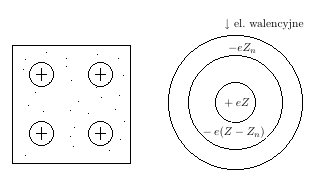
\includegraphics[]{W6_jon.png} \end{center}
\end{enumerate}
\textbf{Gazem Lorenza} nazywamy rozrzedzony gaz, którego cząstki zderzają się 
jedynie ze zlokalizowanymi cenrami rozpraszającymi.
\subsubsection{Aksjomatyczne sformułowanie teorii Drudego-Lorenza}
\begin{enumerate}
\item Atomy metalu ulegają samorzutnej jonizacji, a elekrony walencyjne tworzą 
gaz elektronów przewodnictwa.
\item Elektrony przewodnictwa nie oddziałują wzajemnie, natomiast oddziałuja z 
jonami poprzez zderzenia. Poza zderzeniami ruch elektronu jest opisany 
klasycznie.
\item Zderzenia elektronów z jonami zachodzą z prawdopodobieństwem 
$\frac{1}{\tau}$ w jednostce czasu. W wyniku zderzenia zmienia się jesynie pęd 
elektornu i elektron rozpraszany jest w osowym kierunku.
\item Prędkość rozpraszanego elektronu wynika wyłącznie z lokalnej temperatury
układu.
\end{enumerate}
\subsubsection{Wyprowadzenie Prawa Ohma z teorii D-L}
W ciele stałym występują siły lepkości, które można modelować poniższym wzorem
\begin{equation}
m\ddot{\vec{r}}(t) = -e\vec{E}(t)-m\Gamma \vec{v}(t) - m\Omega^2\vec{r}(t)
\end{equation}
Zał: $\Omega=0$:
\begin{equation}
m\ddot{\vec{r}}(t)=-e\vec{E}(t) - m\Gamma \dot{\vec{r}}(t)
\end{equation}
$$\dim[m\Gamma v]=N = \dim[m]\dim[\Gamma]\dim[v] \implies \dim[\Gamma]=
\dfrac{N}{\frac{kgm}{s}} = \dfrac{1}{s}.$$
Dla zewnętrnego pola $\vec{E}=\vec{0}$: 
\begin{equation}
m\ddot{\vec{r}}(t)+ m\Gamma \dot{\vec{r}}(t)=0
\end{equation}
$$\begin{cases}
\ddot{\vec{r}}(t)=\vec{v}(t) &\\
\ddot{\vec{r}}(t)=-\Gamma \vec{v}(t)
\end{cases} $$
$$\dfrac{d}{dt} [ \ln \vec{v}(t) ] = -\Gamma \implies \vec{v}=\vec{v}_0 
e^{-\Gamma (t-t_0)}$$
$$\tau = \dfrac{1}{\Gamma} \qquad \leftarrow \mbox{śr. czas relaksacji}$$
\begin{center} 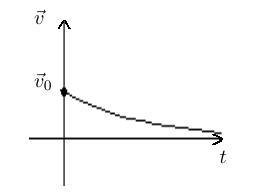
\includegraphics[scale=0.7]{W6_vodt.png}\end{center}
\textbf{Transformata Fouriera}
$$\vec{X}(t) = \dfrac{1}{2\pi} \int_{-\infty}^{\infty} d\omega \vec{X}(\omega)
e^{i\omega t}$$
$$\vec{X}(w) = \dfrac{1}{2\pi} \int_{-\infty}^{\infty} dt \vec{X}(t)
e^{-i\omega t}.$$
Rozważmy $\vec{E} = \vec{E}(t)$. Na poniższe równanie nakładamy obustronnie 
transformatę Fouriera. 
\begin{equation}
\ddot{\vec{r}}(t) = \Gamma \dot{\vec{r}}(t) = -\dfrac{e}{m} \vec{E}(t) 
\end{equation}
$$\dfrac{d^2}{dt^2} \left[ \frac{1}{2\pi} \int_{-\infty}^{\infty} d\omega
\vec{r}(\omega) e^{i\omega t}\right]
+ \Gamma \dfrac{d}{dt} \left[ \frac{1}{2\pi} \int_{-\infty}^{\infty} d\omega
\vec{r}(\omega)e^{i\omega t}\right]=-
\dfrac{e}{m} \frac{1}{2\pi} \int_{-\infty}^{\infty} d\omega \vec{E}(\omega)
e^{i\omega t}
$$
$$\dfrac{1}{2\pi} \int_{-\infty}^{\infty} d\omega \left\{ \left[ 
(i\omega)^2 \vec{r}(\omega) + \Gamma i\omega \vec{r}(\omega)\right]
+ \frac{e}{m}\vec{E}(\omega)\right\}e^{i\omega t}=0$$
$$ \left[ (i\omega)^2 + \Gamma i \omega \right] \vec{r}(\omega) =
-\dfrac{e}{m} \vec{E}(\omega)$$
\begin{equation}
\underline{\vec{r}(\omega) = -\dfrac{e}{m} \dfrac{1}{(i\omega)^2+ 
i\omega\Gamma} \vec{E}(\omega)}.
\end{equation}
Następnie gęstość prądu średniujemy po przestrzeni
$$ \vec{j} \arg = -e \sum_{j/1}^N \vec{v}_j(t)\delta(\vec{r}-\vec{r}_j(t))
\quad / \dfrac{1}{V} \int d^3r$$
$$ \vec{j} (t) = -e\sum_{j/1}^N \vec{v}_j(t) \frac{1}{V}\int d^3r \delta(\vec{r}
- \vec{r}_j(t)) = -e\dfrac{N}{V} \underbrace{\dfrac{1}{N} \sum_{j/1}^N 
\vec{v}_j(t)}_{\vec{v}_{\mbox{śr}}} = -en\vec{v}(t)$$
$$ \vec{j}(t) = -en\dot{\vec{r}}(t).$$
Przechodzimy do reprezentacji fourierowskiej
$$
\vec{j}(\omega) = -eni\omega \vec{r}(\omega)
$$
\begin{equation}
\vec{j}(\omega) = \dfrac{e^2}{m} n \dfrac{i\omega}{(i\omega)^2+i\omega\Gamma} 
\vec{E}(\omega).
\end{equation}
\begin{equation}
\vec{j}(\omega) = \sigma(\omega) \vec{E}(\omega) \qquad \leftarrow 
\mbox{Prawo Ohma (po transformacie F.)}
\end{equation}
$$ \sigma(\omega) = \frac{e^2n}{m} \dfrac{i\omega}{(i\omega)^2+i\omega\Gamma} =
 \frac{e^2n}{m} \dfrac{(-\omega^2-i\omega\Gamma)i
 \omega}{\omega^4+\omega^2\Gamma^2}=\frac{e^2n}{m}\dfrac{\Gamma-
 i\omega}{\omega^2+
 \Gamma^2}  $$
\begin{equation} \sigma(\omega) = \frac{e^2n}{m}\dfrac{\Gamma}{\omega^2+
 \Gamma^2} - i\frac{e^2n}{m}\dfrac{\omega}{\omega^2+\Gamma^2}.\end{equation}
 Niech $\omega=0$:
 $$ \sigma (0) = \frac{e^2n}{m} \frac{1}{\Gamma} =  \frac{e^2n}{m}\tau 
 =\sigma_D $$
 \begin{equation}
 \sigma_D = \dfrac{e^2n}{m} \tau.
 \end{equation}
 \begin{itemize}
 \item jeżeli $\sigma(0) > 0$, to "przewodnik"
 \item jeżeli $\sigma(0) = 0$, to izolator.  
 $\frac{e^2n}{m}\tau=0 $\begin{itemize} \item $n\tau \to 0$ - lokalizacja
 Andersona \item $m\to \infty $ - lokalizacja Motta \end{itemize}
 \end{itemize}
